\vspace{-1pt}
\section{Verification Scaling}
\label{sec:scaling}

Equation~\ref{eq:main} illustrates three independent axes along which verification can be scaled: the granularity of score tokens $G$, the number of repeated evaluations $K$, and the number of evaluation criteria $C$. Each axis targets a different source of error in the reward estimate, and we find that the three act as complementary levers: increasing granularity improves score separation between candidate solutions, repeated evaluation averages out biases from individual verification passes, and criteria decomposition captures complementary aspects of trajectory quality. For all scaling experiments, we use Gemini~2.5~Flash~\citep{gemini25flash} as the verifier, which allows us to extract up to 20 top logprobs per scoring token. In Fig.~\ref{fig:scaling_verifier}, we show that verification accuracy on Terminal-Bench 2.0 improves along all three dimensions, rising from $73.1\%$ at $G{=}1$ to $77.5\%$ at $G{=}20$, from $74.7\%$ at $K{=}1$ to $77.4\%$ at $K{=}16$, and from $75.2\%$--$76.4\%$ for any single criterion to $78.3\%$ when the three criteria are ensembled. We measure the pairwise verification accuracy over 200 randomly sampled trajectories from Terminal-Bench, spanning multiple agent harnesses. Each axis is a knob that the practitioner can tune depending on the latency budget of the downstream application. While our primary experiments use a logprob-accessible model, Appendix~\ref{app:closed-api} demonstrates that our framework is also compatible with frontier models that do not expose token-level log-probabilities via a simple two-stage workaround.

\subsection{Scoring Token Granularity}
\label{sec:granularity}

Standard LM judges collapse the scoring distribution to the single highest-probability token, yielding a discrete reward $R_{\text{LM}}(t,\tau)\in\{1,\ldots,G\}$ with resolution $1/G$. Intuitively, enlarging the ordered token set $V_{\text{score}}$ does not grant the verifier any new information about the trajectory. Yet, it grants the decoder a finer space in which to project the model's internal belief, so that nearby beliefs that would have been rounded to the same integer are now mapped to continuous rewards.

\begin{table}[h!]
    \centering
    \begin{minipage}{0.40\linewidth}
        \centering
        \begin{equation}
        \mathrm{SNR}(G) = \frac{\mathbb{E}[s_c - s_i]}{\sqrt{\mathrm{Var}(s_c - s_i)}}
        \label{eq:snr}
        \end{equation}
    \end{minipage}\hfill
    \begin{minipage}{0.56\linewidth}
        \centering
        \small
        \begin{tabular}{ccccc}
        \toprule
        Granularity $G$ & 1 & 4 & 16 & 20 \\
        \midrule
        SNR ($k{=}16$) & 0.775 & 0.786 & 0.797 & \textbf{0.799} \\
        \bottomrule
        \end{tabular}
    \end{minipage}
    \caption{\textbf{Signal-to-noise ratio (SNR).} \emph{(Left)} The SNR measures how reliably the verifier separates correct ($s_c$) from incorrect ($s_i$) trajectories (Eq.~\ref{eq:snr}). \emph{(Right)} As the number of scoring tokens $G$ increases, the SNR grows, indicating better-calibrated score separation.}
    \label{tab:snr}
\end{table}

\paragraph{Signal-to-Noise Ratio.} To isolate why finer granularity improves verification, we decompose the pairwise score gap $\Delta = s_c - s_i$ between correct ($s_c$) and incorrect ($s_i$) trajectories into a signal and a noise component. We define the signal-to-noise ratio as in Eq.~\ref{eq:snr} (Table~\ref{tab:snr}, left), where $\mathbb{E}(s_c-s_i)$ captures how strongly the verifier prefers the correct trajectory over the incorrect one (\emph{signal strength}), and the denominator, $\mathrm{Var}(s_c - s_i)$, captures how inconsistent that preference is across pairs (\emph{noise}). Pairwise verification accuracy is a monotonic function of $\mathrm{SNR}(G)$: holding sample size fixed, a larger standardized gap implies a higher probability that $s_c>s_i$. Empirically, we find that $\mathrm{SNR}(G)$ increases from $0.775$ at $G{=}1$ to $0.799$ at $G{=}20$ on Terminal-Bench (Table~\ref{tab:snr}). Finer-grained tokens therefore produce better-calibrated scores that more reliably separate correct from incorrect trajectories, which in turn improves the pairwise accuracy from $73.1\%$ to $77.5\%$.

\vspace{-0.15in}
\paragraph{Case Study: \texttt{query-optimize}.}
To concretely illustrate how scaling granularity to $G{=}20$ and our probabilistic formulation sharpen the verifier's signal, we analyze a representative trajectory pair from the \texttt{query-optimize} task on Terminal-Bench~V2, generated by Claude~Opus~4.5 under the OpenHands harness and scored by Gemini~2.5~Flash. Here the agent is given a slow SQL query over a database and asked to produce an equivalent optimized version. Both candidate trajectories generate queries that execute faster, but they differ critically in their verification procedures. The correct trajectory waits the full $5$ minutes for the original query to complete on the canonical database and performs a direct \texttt{diff} against the optimized output. In contrast, the failing trajectory never validates equivalence on the database and instead creates a new database. As shown in the reasoning traces in Appendix~\ref{app:query-optimize-example}, Gemini~2.5~Flash reliably identifies this failure mode, but expresses it in graded, hedged language (e.g., \textit{``slightly cleaner,''} \textit{``marginally more direct''}), as if the discrepancy were minor. When evaluated over 100 repetitions, a standard LM judge on a $1$--$5$ scale collapses these nuanced assessments into discrete scores (Table~\ref{tab:query-optimize-main}), producing ties (e.g., $5$ vs.\ $5$) in $88$ out of $100$ runs, thus failing to meaningfully discriminate between the candidates. Taking the expectation over the \emph{same} $5$-point distribution eliminates ties entirely---ranking the correct trajectory higher in $69$ runs---and scaling the granularity to $G{=}20$ sharpens the signal further, letting LLM-as-a-Verifier rank the correct trajectory strictly higher in $77$ out of $100$ runs.

\begin{table}[h!]
    \centering
\caption{\textbf{Judges vs.\ Verifiers on \texttt{query-optimize}.} Over $100$ repeated evaluations, we count how often the correct trajectory is scored higher than ($s_c{>}s_i$), tied with ($s_c{=}s_i$), or lower than ($s_c{<}s_i$) the incorrect one. The discrete $1$--$5$ judge produces ties in $88/100$ evaluations. Taking the expectation over the same $1$--$5$ scale eliminates ties and correctly ranks the trajectory in $69/100$ evaluations. Increasing the score granularity to $G{=}20$ further improves discrimination, correctly ranking the trajectory in $77/100$ evaluations.}
    \label{tab:query-optimize-main}
    \small
    \renewcommand{\arraystretch}{1.3}
    \begin{tabular}{llccc}
    \toprule
    Method & Reward $R(x,\tau)$ & $\#(s_c{>}s_i)$\,{\color{deepgreen}\cmark} & $\#(s_c{=}s_i)$~\textbf{\textit{(tie)}} & $\#(s_c{<}s_i)$\,{\color{deepred}\xmark} \\
    \midrule
    Judge (discrete, $G{=}5$)        & $\phi\!\left(\arg\max_g p_{\theta}(v_g)\right)$       & $12/100$ & $88/100$ & $0/100$ \\
Verifier (continuous, $G{=}5$)
& $\sum_{g=1}^{5} p_{\theta}(v_g)\,\phi(v_g)$
& $69/100$ & $0/100$ & $31/100$ \\

\textbf{Verifier (continuous, $G{=}20$)}
& $\sum_{g=1}^{20} p_{\theta}(v_g)\,\phi(v_g)$
& $\mathbf{77/100}$ & $\mathbf{0/100}$ & $23/100$ \\
    \bottomrule
    \end{tabular}
\end{table}

\subsection{Repeated Evaluation}
\label{sec:repeated}

While granularity improves score calibration within a single forward pass, it does not address a second source of error: the verifier's variance on one evaluation. Even at high $G$, a single evaluation $R^{(k)}(x,\tau)$ can be skewed by spurious features of the prompt or failure modes of the verifier on a particular trajectory. Averaging $K$ independent evaluations $\frac{1}{K}\sum_{k=1}^{K} R^{(k)}(x,\tau)$ is a Monte Carlo estimator of the underlying expected reward; its variance shrinks as $\mathcal{O}(1/K)$ while its bias is unchanged. This complements granularity rather than duplicating it: granularity sharpens each individual estimator, while repeated evaluation averages out the noise that granularity cannot remove. Fig.~\ref{fig:scaling_verifier} (middle) shows that the accuracy increases from $74.7\%$ at $K{=}1$ to $77.5\%$ at $K{=}16$. However, gains diminish with larger $K$: early improvements arise from variance reduction, while additional evaluations contribute diminishing returns due to correlated biases on harder examples. Importantly, repeated evaluation benefits discrete judges, whose coarse scoring induces high tie rates at low $K$. While increasing $K$ helps break these ties through averaging, this mechanism is fundamentally limited for discrete judges. We show that a single-pass verifier ($K{=}1$) already matches a heavily ensembled judge ($K{=}16$), highlighting that fine-grained probabilistic scoring provides a stronger signal.

\begin{figure}[t]
    \centering
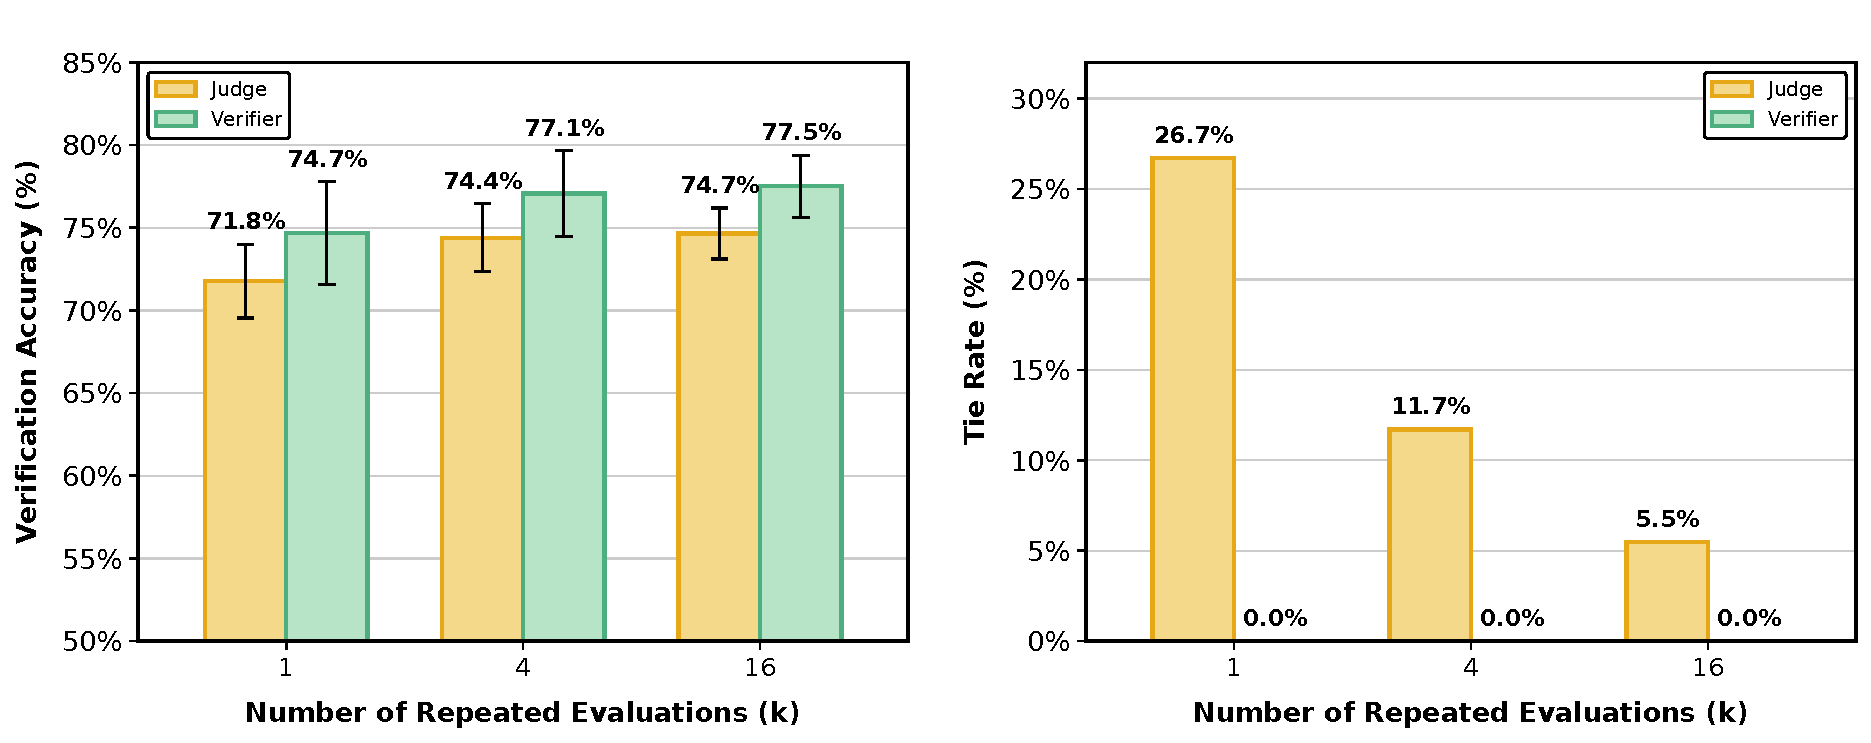
\includegraphics[width=\linewidth]{figures/judge_vs_verifier.pdf}
    \caption{\textbf{Verifier (continuous) vs.\ Judge (discrete)} on Terminal-Bench~V2 across $k \in \{1, 4, 16\}$ repeated evaluations.
    \textbf{Left:} Pairwise verification accuracy. The verifier achieves $74.7\%$ at $k{=}1$ and improves to $77.5\%$ at $k{=}16$, consistently outperforming the judge across all evaluation budgets. 
    \textbf{Right:} Tie rate. The judge produces ties in $26.7\%$ of comparisons at $k{=}1$ due to coarse discrete scoring, decreasing to $5.5\%$ at $k{=}16$ as averaging breaks ties. In contrast, the verifier yields zero ties.}
    \label{fig:judge_verifier}
\end{figure}

\subsection{Criteria Decomposition}
\label{sec:criteria}

Granularity and repeated evaluation both assume that the rubric itself is adequate; neither helps if a single monolithic criterion is a poor proxy for trajectory quality. In long-horizon agentic tasks, judgments like ``is this trajectory correct?'' conflate several logically distinct factors, and verifiers asked a compound question often latch onto whichever factor is most salient in the prompt. Therefore, we replace a single monolithic rubric with an ensemble over $C$ simpler sub-criteria. Concretely, for code-agent trajectories we decompose correctness into three factors that are individually easier to verify: Specification (whether the trajectory satisfies all task requirements), Output (whether the final output format matches the expected result), and Errors (whether the trajectory is free of failure signals in logs and tool outputs). The final reward averages the expected scores across criteria, as in the outer sum of Eq.~1. In Fig.~\ref{fig:scaling_verifier} (right), any one criterion alone achieves $75.2\%$--$76.4\%$ accuracy, and their ensemble reaches $78.3\%$.